\section{Experiment}

Table \ref{table:heatmap} summarizes our results. We list our results in order of parameter numbers in the model. This is a combination of trainable and untrainable parameters, as the core architecture of our models is generally a flavor of a recurrent neural network sequence-to-sequence model. The core architectural differences are captured by the method we use for embedding words and colors, while our encoder-decoder architecture generally stays the same. We use GRU as a default cell for all experiments. We also used an LSTM cell for the experiments that have shown best model performance to evaluate how a LSTM affects the performance of the models in comparison with GRU.

\par
We experimented with four different hidden dimensions for the RNN cells. We used 50 (default for all experiments), 100, 150, 250 to determine what hidden dimensions will have the most positive effect on the model performance. Those experiments were conducted on models with RoBERTa, BERT, XLNet or ELECTRA pre-trained word embeddings and Fourier transformed or ResNet concatenated with Fourier transformed color embeddings. A subset of the train dataset (8,000 records) was used for those experiments. We limited the number of experiments due to time and budget constraints. Finally, we trained and tested the best performing models with a hidden dimension of 250 as our experiments showed that a higher dimension has a positive effect on the model output.

\par
For example, for our simplest model we use a Fourier transformation to project the colors from a 3-dimensional vector to a 54-dimensional vector. We use 50-dimensional pre-trained GloVe embeddings to embed each word in the corpus as a distributed representation. We use a sequence-to-sequence model with a GRU cell acting as a color encoder and text decoder.  For this baseline model (and all models) we set the hidden dimension of the GRU to 50. From \citep{dey-2017-gru} there are a total of:
\begin{equation}
  3*(n^2 + n*m +n)
\end{equation}
where \(n\) is the hidden dimension of the GRU and \(m\) is the input dimension to the cell. So for our encoder our number of trainable weights becomes:
\begin{equation}
  3*(50^2 + 50*54 +50) = 15,150
\end{equation}
and for the decoder our number of weights becomes:
\begin{equation}
  3*(50^2 + 50*50 +50) = 15,750
\end{equation}

For the entire architecture this totals to 30,900 trainable parameters. We note that we freeze the word embeddings and color embeddings in all models.

\par
For a more complex model that incorporates both transformer pre-trained or contextual word embeddings and color embeddings generated by a convolutional encoder, our number of trainable parameters increases. For a model that uses 768-dimensional BERT embeddings and 512-dimensional ResNet encoded color embeddings our trainable parameters for the encoder becomes:
\begin{equation}
  3*(50^2 + 50*512 +50) = 84,450
\end{equation}
and for the decoder our number of weights becomes:
\begin{equation}
  3*(50^2 + 50*768 +50) = 122,850
\end{equation}

\par
This results in a total of 207,300 trainable parameters. The number of trainable parameters significantly increases for the experiments where we used hidden dimension of 250. For the aforementioned example the number of trainable parameters used in the encoder becomes:
\begin{equation}
  3*(250^2 + 250*512 +50) = 571,650
\end{equation}
and for the decoder the number of weights becomes:
\begin{equation}
  3*(250^2 + 250*768 +50) = 763,650
\end{equation}

\par
We note that while the more complex models have more power to capture complex interactions, the large models have nearly seven times the number of trainable parameters leading to concerns of building models with high variance. We will discuss the effects of model size and overfitting further in our analysis section.

\par
For all models we stop training after the validation performance has increased for 10 iterations in a row at a tolerance of \(10^{-5}\). We use the listener accuracy and the BLEU score to evaluate model performance.

\par
Listener accuracy and BLEU score are used for evaluating the performance of the models. The former allows us to evaluate the ability of the trained model to construct accurate color description utterances based on the colors input:
\begin{equation}
  c^{*} = argmax_{c \in C} P_{s} (utterance | c)
\end{equation}
where \(P_{s}\) is the describer model and \(C\) is the set of all permutations of all three colors in the color context. We take \(c^{*}\) to be a correct prediction if it is one where the target is in the privileged final position \citep{potts-2020-colors}.

\par
The listener's accuracy assesses the ability of the model to communicate with itself and this can lead to generating utterances that are far from proper English. BLEU score is used to ensure that this situation doesn’t happen.

\par
We consider both listener accuracy and BLEU score, with equal weight when evaluating the models and therefore, a model is consider better performing if both scores are higher.

\begin{table*}[ht]
\centering
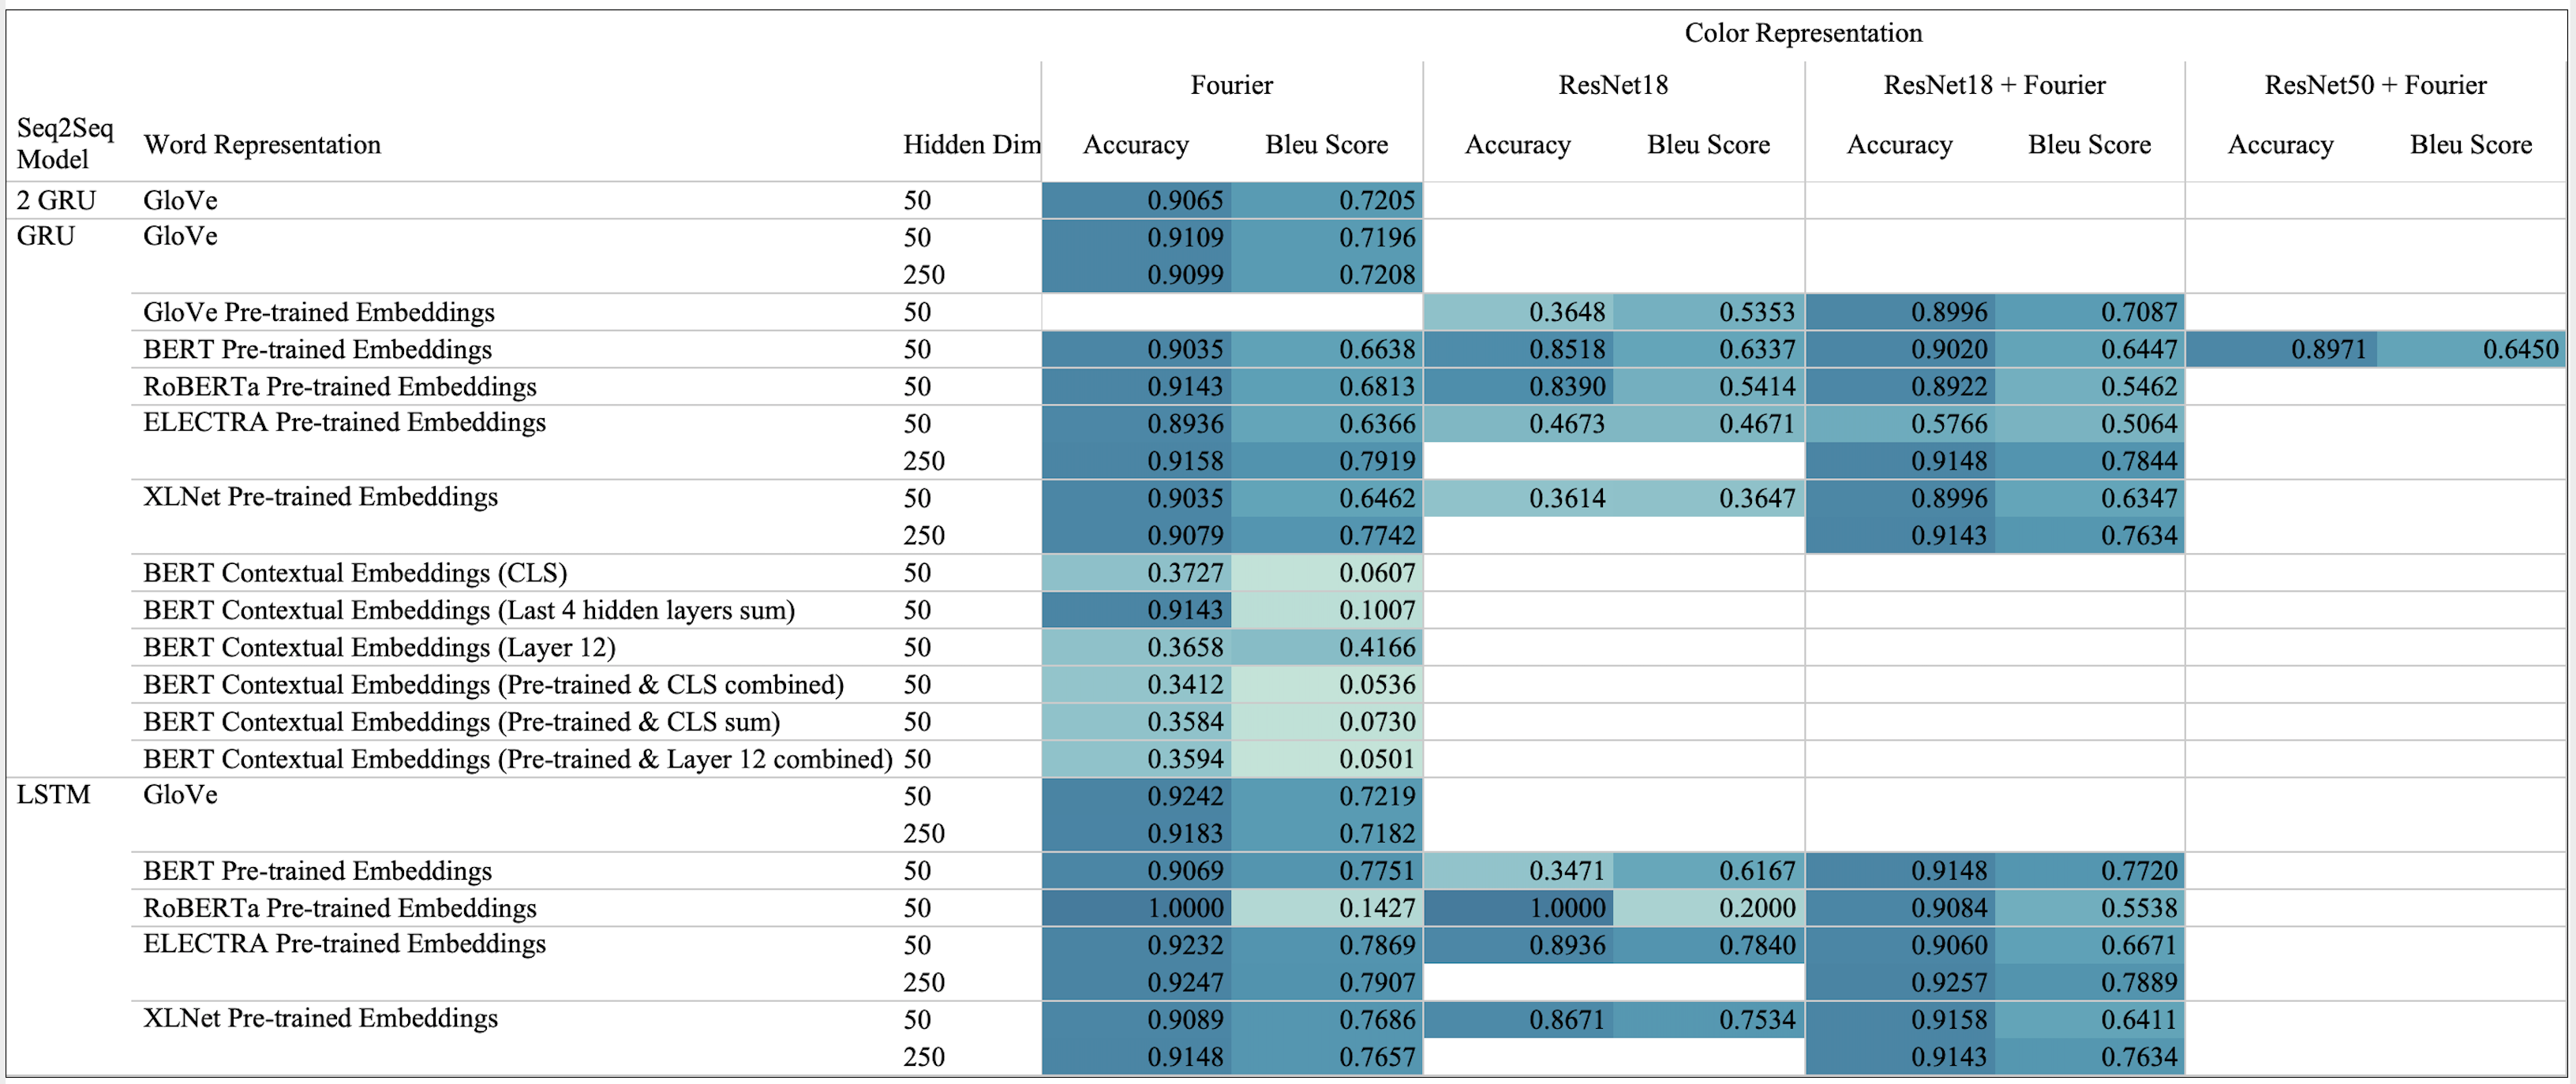
\includegraphics[width=\textwidth]{assets/heatmap.pdf}
\caption[Heatmap]{Heatmap with all experiment results. The darker the color the better the performance of the model. The best performing architectures are based on ELECTRA and XLNet pre-trained word embeddings with ResNet-18 combined with Fourier color representations.}
\label{table:heatmap}
\end{table*}
